\documentclass[11pt,a4paper]{article}
\usepackage[T1]{fontenc}
\usepackage[utf8]{inputenc}
\usepackage{lmodern,microtype}
\usepackage{amsmath,amssymb,amsthm,mathtools,bm}
\usepackage{booktabs,array,tabularx,longtable}
\usepackage{graphicx,float,caption}
\usepackage{xcolor}
\usepackage[margin=20mm]{geometry}
\usepackage{enumitem,fancyhdr}
\usepackage[hidelinks]{hyperref}
\hypersetup{
 pdftitle={FIN ST82--ST93: Projection Fibers, Passive Time, and Falsification},
 pdfauthor={Krzysztof Żuchowski},
 pdfsubject={Analytical and computational execution of FIN programs ST82--ST93},
 pdfkeywords={FIN, projection, conditional expectation, nonidentifiability, passive memory, spin lift, CPTP, thermodynamics, symmetry breaking}
}
\setlength{\parindent}{0pt}
\setlength{\parskip}{0.48em}
\setlength{\emergencystretch}{2em}
\setlength{\headheight}{14pt}
\setlist[itemize]{leftmargin=1.55em,itemsep=0.14em,topsep=0.2em}
\setlist[enumerate]{leftmargin=1.75em,itemsep=0.14em,topsep=0.2em}
\pagestyle{fancy}\fancyhf{}
\lhead{FIN ST82--ST93}\rhead{Release 10.61}\cfoot{\thepage}
\newtheorem{theorem}{Theorem}[section]
\newtheorem{proposition}[theorem]{Proposition}
\newtheorem{corollary}[theorem]{Corollary}
\newcommand{\proven}{\textcolor{green!40!black}{\textbf{[PROVEN]}}}
\newcommand{\strong}{\textcolor{blue!70!black}{\textbf{[STRONG EVIDENCE]}}}
\newcommand{\moderate}{\textcolor{cyan!45!black}{\textbf{[MODERATE EVIDENCE]}}}
\newcommand{\conditional}{\textcolor{violet!65!black}{\textbf{[CONDITIONAL]}}}
\newcommand{\blocked}{\textcolor{red!72!black}{\textbf{[NOT CLOSED]}}}
\newcommand{\statusboundary}{\textcolor{orange!80!black}{\textbf{[BOUNDARY]}}}
\newcommand{\resultbox}[1]{\begin{center}\fcolorbox{blue!60!black}{blue!4}{\parbox{0.92\textwidth}{#1}}\end{center}}

\begin{document}
\pagenumbering{gobble}
\begin{titlepage}
\centering
\vspace*{1.1cm}
{\LARGE\bfseries FIN ST82--ST93\par}
\vspace{0.35cm}
{\Large Projection Fibers, Passive Time, and Falsification of the ``Projected Universe'' Hypothesis\par}
\vspace{0.42cm}
{\large Exact coarse quotients, hidden-lift nonidentifiability, spin-boundary classes, passive memory, reversible faces, thermodynamic separation, nonlinear branches, and a claim-level dependency graph\par}
\vspace{0.95cm}
{\Large Krzysztof Żuchowski\par}
\vspace{0.24cm}
{\large Independent Researcher --- Fractal Information Theory Project\par}
{\large ORCID: 0009-0002-0909-3613\par}
\vspace{0.75cm}
{\large FIN Release 10.61 --- Version 1.0.0\par}
{\large August 11, 2026\par}
\vfill
\begin{minipage}{0.90\textwidth}
\textbf{Research question.} Assume only as a counterfactual hypothesis that observable reality is an internal projection or operational quotient of a deeper FIN object. Does present FIN mathematics derive that projection, or merely permit examples of it?\par
\textbf{Method.} Finite operator identities, spectral functional calculus, exact analytic no-go theorems, finite $C^*$-algebra structure, an explicit Gibbs-preserving counterexample, local nonlinear continuation, robust synthetic likelihood optimization, and twenty-three live tests.\par
\textbf{Epistemic rule.} Mathematical compatibility with a projection picture is not evidence that the physical universe is such a projection. A hidden-variable fiber is not an ontological layer below the nadsoliton; within FIN terminology the nadsoliton remains the primordial fractal information in a solitonic state.\par
\textbf{Repository snapshot.} Git commit \texttt{dc6f8f924d1636af284f386d145103eb694c2034}; the working tree also contains the local artifacts listed in the release manifest.\par
\textbf{Repository.} \url{https://github.com/hyconiek/Fractal-Nadsoliton-Theory}\par
\textbf{License.} CC BY 4.0.
\end{minipage}
\end{titlepage}
\pagenumbering{arabic}

\begin{abstract}
This report executes ST82--ST93 and subjects the ``projected universe'' reading of FIN to a direct falsification program. Its main positive result is exact but double-edged. For every nonnegative fine parameter $q$, the declared dyadic lift $A_{24}(q)$ has a reducing coarse sector with isometry
\[
P=2^{-1/2}(I,I)^T,
\qquad P^*A_{24}(q)P=A_{12},
\qquad P^*A_{24}(q)F=0,
\]
where $F=2^{-1/2}(I,-I)^T$. Consequently
\[
P^*f(A_{24}(q))P=f(A_{12})
\]
for every spectral function $f$. Heat, unitary, Green, wave, and other functional-calculus channels are therefore exactly identical after coarse compression, while the complementary fine block changes with $q$. FIN thus possesses a rigorous finite model of a deeper object projecting to the same observable dynamics. The same theorem proves nonidentifiability: infinitely many inequivalent deeper lifts cast the identical complete coarse spectral ``shadow.'' Nothing in coarse $A_{12}$ selects $q$ or proves that physical reality uses this quotient.

ST84 proves that the certified positive-pole, positive-residue memory is passive and completely monotone. It cannot itself generate active positive gain or a temporal selector. ST85 classifies the periodic and antiperiodic spin-boundary classes; the half-angle lift exists only after boundary/state data are supplied. ST88 proves that every ST75 full-space intertwiner is irreversible because it factors through a pinching with 122-dimensional kernel, while the quotient algebra $\mathbb C\oplus M_2^5\oplus\mathbb C$ has reversible $*$-automorphisms. ST89 gives an explicit Gibbs-preserving channel that is not a thermal operation, proving that Gibbs preservation alone does not provide physical thermodynamic dynamics.

ST83 reproduces the ST77 fold at $\kappa=0.016589052386382905$ with stable floating transversality, but fails to produce the requested outward interval certificate. ST87 obtains a robust synthetic Chernoff rate under declared contamination. ST90 finds many reflection-reduced stationary signatures but is not exhaustive. ST91 proves a conditional local exchange of stability for the constructed twelve-branch potential. ST92 proves that powers of strict $A$, their diagonal contractions, and their polynomial commutators contain no reflection-odd selector. ST93 exports a machine-readable dependency DAG. The verdict is precise: a projection interpretation is mathematically coherent and now has an exact internal example, but the physical projection map, selector, boundary class, clock, dimensional unit, preparation, instrument, and independent record remain unsourced.
\end{abstract}

\textbf{Status vocabulary.} \proven{} means an exact finite or analytic result in the declared class. \strong{} and \moderate{} mean numerical evidence without an interval/global theorem. \conditional{} means exact only after displayed added premises. \blocked{} means that the stated target was attempted but not certified. \statusboundary{} records a non-implication.

\tableofcontents
\newpage

\section{Frozen mathematical core and the counterfactual hypothesis}

The strict working object is the graph Laplacian on $C_{12}$
\begin{equation}
W_{xx}=0,\qquad
W_{xy}=\frac{\cos(0.18575d(x,y)+0.16250)}{1+d(x,y)^{1.8}}\quad(x\ne y),
\qquad A=sI-W,
\label{eq:strict}
\end{equation}
with $s=1.660307278766099$ to the displayed precision. Thus
\[
\langle f,Af\rangle=\frac12\sum_{x,y}W_{xy}|f_x-f_y|^2\ge0.
\]
The zero diagonal is part of the definition. The legacy ontological kernel remains an intermediate bridge kernel. No legacy physical-role formula is transferred to~\eqref{eq:strict} in this report.

We formalize the user's suggestion as a counterfactual:
\begin{equation}
\mathbf H_{\rm PROJ}:\quad
\text{observable reality is an operational projection or quotient of a deeper FIN realization.}
\end{equation}
This hypothesis has three logically independent clauses:
\begin{enumerate}
\item a deeper object and a mathematically defined coarse map exist;
\item FIN selects that object and map rather than merely allowing them;
\item the quotient is connected to calibrated physical observations.
\end{enumerate}
ST86 proves a strong version of clause 1 for a finite model. It refutes uniqueness in clause 2. Clause 3 remains open.

The word ``deeper'' here denotes a finer representation of the nadsoliton, not a new informational substance below it. This preserves the FIN ontology
\[
\text{nadsoliton}\longrightarrow\text{light}\longrightarrow\text{matter}\longrightarrow\text{emergent observer}.
\]

\resultbox{\textbf{Central result.} FIN contains an exact projection fiber, not a derived projected universe. The fine-to-coarse map preserves all spectral-functional dynamics, but its fiber is nontrivial and unidentifiable from the coarse record. Projection is therefore a mathematically admissible architecture and simultaneously an underdetermined physical interpretation.}

\section{Outcome matrix}
\small
\begin{longtable}{@{}p{0.055\textwidth}p{0.30\textwidth}p{0.24\textwidth}p{0.31\textwidth}@{}}
\toprule
ID & Object & Result & Boundary\\
\midrule\endfirsthead
\toprule ID & Object & Result & Boundary\\\midrule\endhead
ST82 & Independent ST58 regeneration & \blocked{} rational implementation stopped locally & ST70 exact replay remains valid; no independent upstream regeneration\\
ST83 & Fold interval certificate & \strong{} simple-fold evidence & No outward 15-variable Krawczyk proof\\
ST84 & Passive memory and time & \proven{} complete-monotonicity no-go & External nonequilibrium/time order may evade\\
ST85 & $C_{24}$ spin boundary & \proven{} classification, \conditional{} realization & Strict scalar data do not choose a class\\
ST86 & Dyadic projection fiber & \proven{} exact quotient and nonidentifiability & No physical projection theorem\\
ST87 & Robust likelihood & \strong{} declared synthetic nuisance optimum & Not calibrated laboratory performance\\
ST88 & Reversible faces & \proven{} full/quotient separation & No physical measurement map derived\\
ST89 & GP versus thermal maps & \proven{} explicit counterexample & Bath and energy scale remain added\\
ST90 & Disconnected branches & \moderate{} multistart inventory & Finite search is not exhaustive\\
ST91 & Dynamic backreaction & \proven{} conditional local bifurcation & Potential, metric and clock inserted\\
ST92 & Reflection-odd source & \proven{} no-go in declared class & Nonlinear state/boundary tensors remain outside\\
ST93 & Dependency schema & \proven{} acyclic audit graph & Graph consistency is not physical evidence\\
\bottomrule
\end{longtable}
\normalsize

\section{ST82--ST83: certification boundary}

\subsection{ST82 --- independent regeneration attempt}

ST70 had already checked the serialized ST58 acceptance inequalities using exact \texttt{Fraction} arithmetic, but retained the upstream transcendental intervals as trusted inputs. ST82 implemented a more ambitious, independent route: Machin's formula for $\pi$, alternating rational arctangent intervals, rational Taylor bounds for trigonometric functions, exact integer fifth-root bracketing for $d^{9/5}$, rational Fourier enclosures, and rational Krawczyk inequalities.

The local implementation was deliberately stopped after it exceeded the bounded runtime suitable for this batch. It produced no certificate file. This is an implementation/performance failure, not a counterexample and not an invalidation of ST58. The accepted status is therefore:
\[
\boxed{\text{ST70 exact replay survives; ST82 independent regeneration remains open.}}
\]
No result is promoted from the unfinished calculation.

\subsection{ST83 --- the first nonlinear fold}

ST83 independently refines the 15-equation fold system consisting of seven stationary equations, seven null-vector equations, and one normalization equation. It recovers
\[
\kappa_{\rm fold}=0.016589052386382905,
\]
with maximum residual at double precision below the stored tolerance. Central finite-difference Jacobians over steps $10^{-4}$ through $3\times10^{-7}$ give minimum singular values bounded below numerically by
\[
\sigma_{\min}>0.08024666.
\]
This is stable numerical transversality evidence, not an interval lower bound.

\begin{figure}[H]\centering
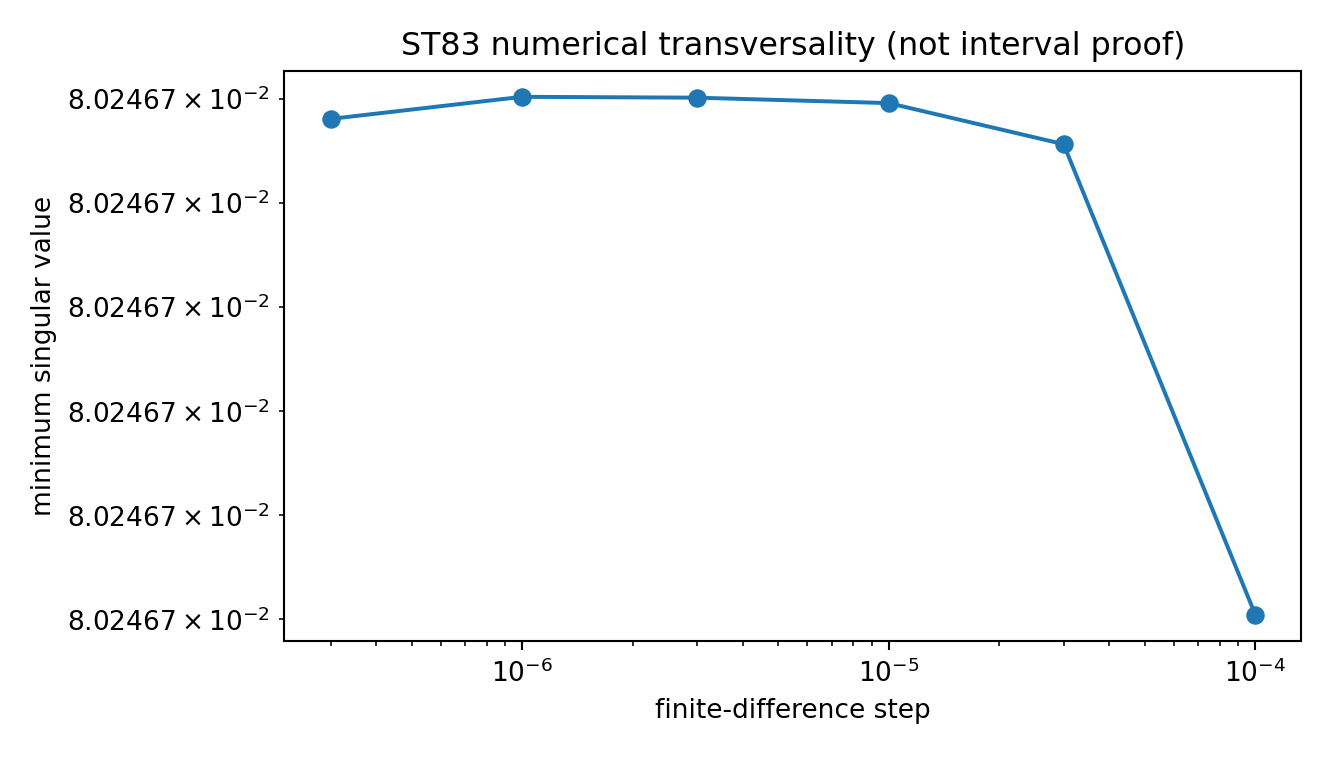
\includegraphics[width=0.70\textwidth]{FIN_ST82_ST93_Figures/st83_fold_attempt.png}
\caption{The numerical transversality indicator is stable across finite-difference scales. No outward interval Jacobian was produced, so the result remains strong numerical evidence.}
\end{figure}

\section{ST84: why passive memory does not create the time arrow}

The certified memory response has Stieltjes form
\begin{equation}
M(z)=\sum_{j=1}^{6}\frac{r_j}{z+p_j},\qquad p_j>0,\quad r_j>0.
\label{eq:stieltjes}
\end{equation}
Its impulse response is
\[
m(t)=\sum_j r_j e^{-p_jt}.
\]
For every integer $n\ge0$,
\begin{equation}
(-1)^n m^{(n)}(t)=\sum_j r_jp_j^n e^{-p_jt}>0.
\label{eq:cm}
\end{equation}

\begin{theorem}[Passive-memory obstruction]
Every memory kernel of form~\eqref{eq:stieltjes} is completely monotone and positive real. It stores and dissipates response but cannot supply active positive gain or select a temporal orientation by itself.
\end{theorem}

The proof is the displayed identity~\eqref{eq:cm}; positivity of the certified pole and residue intervals pays every term. A time-oriented amplifier therefore needs at least one resource outside this passive class: a pump, a nonequilibrium population, a signed/active residue, a boundary condition, or an oriented preparation/record. This sharpens the earlier intuition that memory plus feedback might automatically produce time. Passive memory produces retardation, not a strict arrow.

\begin{figure}[H]\centering
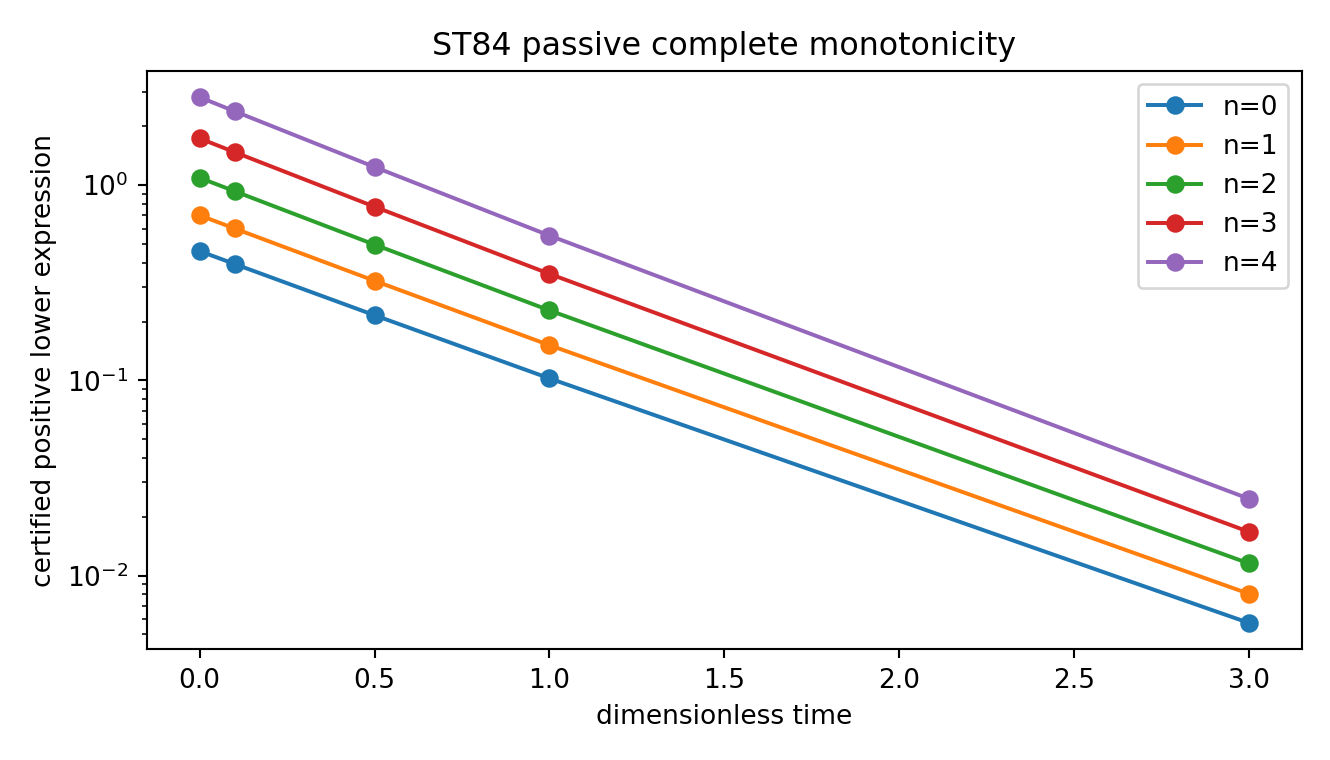
\includegraphics[width=0.72\textwidth]{FIN_ST82_ST93_Figures/st84_passive_memory.png}
\caption{Positive lower expressions for the first five signed derivatives in~\eqref{eq:cm}. The plotted samples illustrate an analytic all-time theorem.}
\end{figure}

The result also corrects the loose statement that a soliton's frequency already supplies physical time. The unitary phase $e^{-itA}$ gives a dimensionless phase parameter. Under $(A,t)\mapsto(cA,t/c)$ it is unchanged. Wave evolution $\cos(t\sqrt A)$ has the different scaling $(A,t)\mapsto(cA,t/\sqrt c)$. Frequency ratios are internal; seconds require a clock calibration and a channel-specific dimensional map.

\section{ST85: projective spin exists, but its source does not}

A cyclic system admits two $\mathbb Z_2$ spin boundary classes:
\[
\psi(x+12)=+\psi(x),\qquad \psi(x+12)=-\psi(x).
\]
Their momenta are respectively
\[
k_n=\frac{2\pi n}{12},\qquad
k_{n+1/2}=\frac{2\pi(n+1/2)}{12}.
\]
The second class is naturally represented on the central extension $C_{24}\to C_{12}$ and exhibits the half-angle/projective behavior discussed in earlier programs.

\begin{proposition}[Lift nonselection]
The real scalar, dihedral-invariant operator $A$ determines neither the periodic versus antiperiodic boundary class nor an oriented section of the $C_{24}$ cover.
\end{proposition}

Existence and selection must not be conflated. A supplied boundary state can realize the projective sector. The strict scalar core does not generate that boundary state. The result therefore supports the projection picture only conditionally: a richer state can project to the scalar quotient, but the rich state is not yet derived.

\section{ST86: the exact projection-fiber theorem}

Let $A_{24}(q)$ be the declared dyadic lift of $A_{12}$, with $q\ge0$ the new fine antipodal weight. Define isometries
\[
P=\frac1{\sqrt2}\begin{pmatrix}I\\I\end{pmatrix},\qquad
F=\frac1{\sqrt2}\begin{pmatrix}I\\-I\end{pmatrix}.
\]
The periodic embedding identity from the refinement construction is
\[
A_{24}(q)P=PA_{12}.
\]
Since $A_{24}(q)$ is self-adjoint and the complementary sector is invariant under the half-cycle exchange,
\begin{equation}
P^*A_{24}(q)P=A_{12},\qquad P^*A_{24}(q)F=0.
\label{eq:block}
\end{equation}

\begin{theorem}[Projection fiber]
For every Borel function $f$ defined on the finite spectrum,
\begin{equation}
P^*f(A_{24}(q))P=f(A_{12})
\label{eq:functional}
\end{equation}
for every $q\ge0$. The complementary block $F^*A_{24}(q)F$ varies with $q$.
\end{theorem}

\textit{Proof.} Equation~\eqref{eq:block} is a reducing block decomposition. Finite-dimensional spectral functional calculus acts blockwise, giving~\eqref{eq:functional}. Direct inspection of the lift shows that the fine antipodal term changes only the complementary block. \hfill$\square$

The theorem simultaneously covers
\[
e^{-itA},\quad e^{-tA},\quad(A+zI)^{-1},\quad\cos(t\sqrt A),\quad e^{-\beta A},
\]
subject to each channel's own nuisance parameter and dimensional interpretation. Sampled residuals are $1.4\times10^{-15}$ or below, while the maximum sampled fine-block difference is $10.3923$. Normalization requires care: $P^*e^{-\beta A_{24}}P=e^{-\beta A_{12}}$, but the global partition function $Z_{24}(q)$ varies with the fine block. Thus a globally normalized 24-state Gibbs state assigns a $q$-dependent total probability to the coarse sector. Only after conditioning on that sector and renormalizing does one recover the 12-state Gibbs state exactly.

\begin{figure}[H]\centering
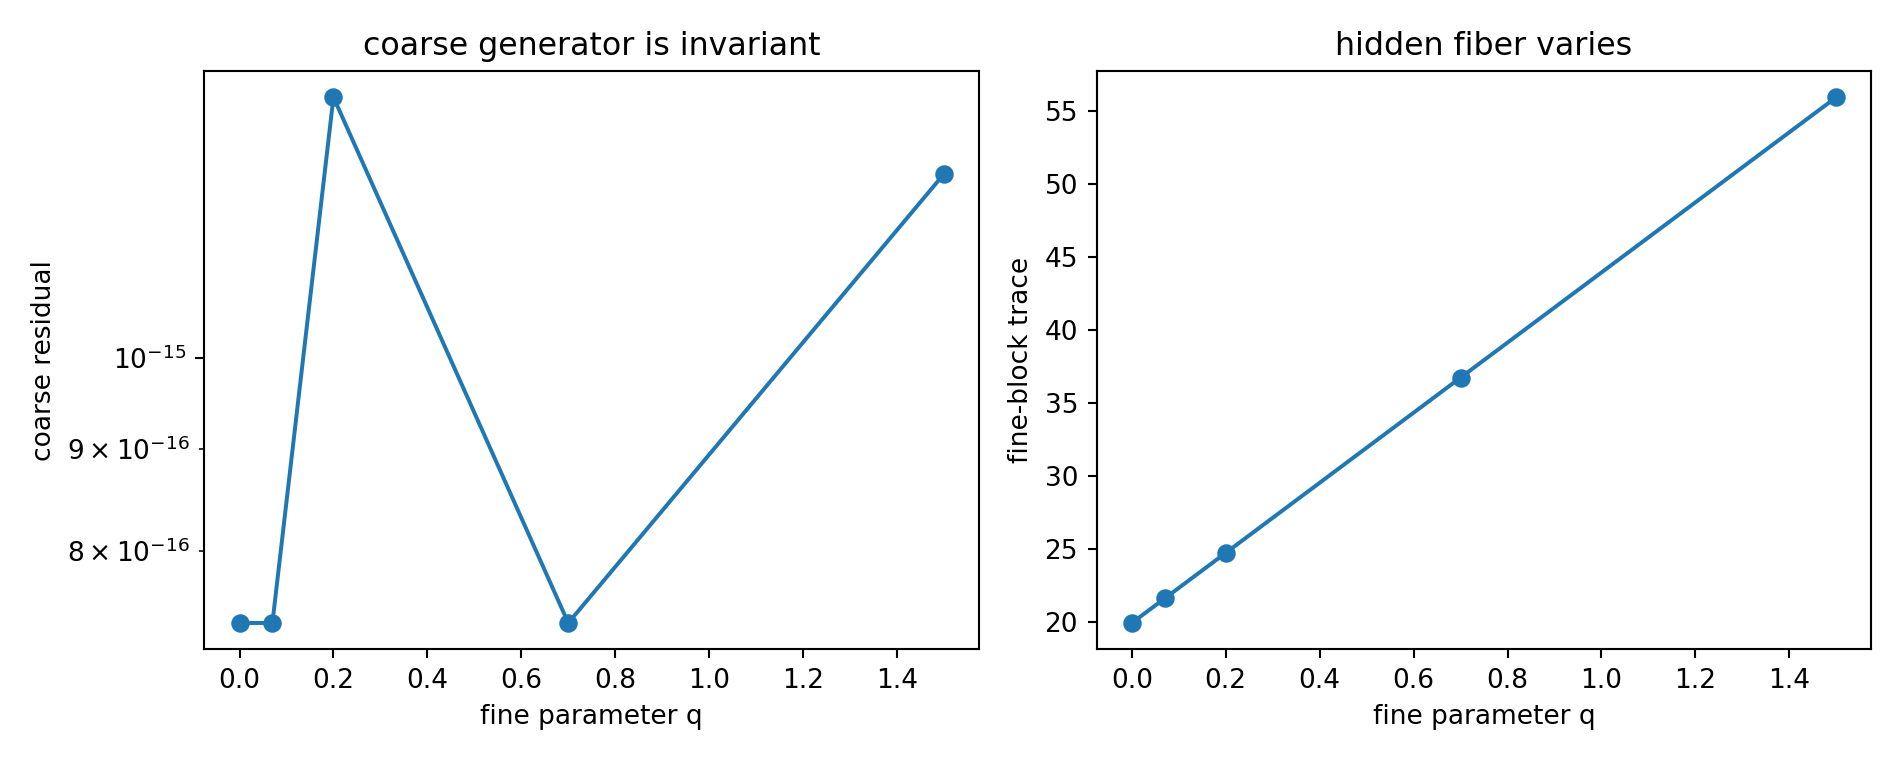
\includegraphics[width=0.90\textwidth]{FIN_ST82_ST93_Figures/st86_projection_fiber.png}
\caption{Left: the coarse generator is invariant to floating precision. Right: the hidden fine block varies strongly with $q$.}
\end{figure}

\begin{corollary}[Nonidentifiability]
No experiment restricted to the complete coarse functional-calculus algebra, conditioned entirely inside $P\mathcal H$ and without access to its global occupation probability, can identify $q$. Infinitely many inequivalent fine generators have identical coarse heat, unitary, wave, Green, and unnormalized Boltzmann records. A measurement of the coarse-sector weight in a globally normalized Gibbs ensemble lies outside this restricted record and can depend on $q$.
\end{corollary}

This is the most important result of the batch. It supplies the first sharp answer to the proposed intuition:
\begin{itemize}
\item \textbf{Supported mathematically:} one deeper FIN realization can project to a lower-dimensional observable dynamics; a small spectral core can generate many channel shadows.
\item \textbf{Falsified as a uniqueness claim:} the observable shadow does not determine its deeper generator.
\item \textbf{Not addressed physically:} no result identifies the coarse sector with our universe, selects $q$, or constructs an apparatus that measures only $P\mathcal H$.
\end{itemize}

Thus ``the universe is a FIN projection'' is not presently a prediction. Without a new selection or sufficiency axiom it is an equivalence class of possible models.

\section{ST87: robust synthetic likelihood}

ST87 replaces a coarse concentration estimate by a direct nuisance optimization for the declared synthetic two-carrier probability tables. Each distribution is independently contaminated by a uniform component,
\[
p_{\epsilon_P}=(1-\epsilon_P)p+\epsilon_Pu,
\quad q_{\epsilon_Q}=(1-\epsilon_Q)q+\epsilon_Qu,
\quad 0\le\epsilon_P,\epsilon_Q\le0.12.
\]
The Chernoff information is
\[
C(p,q)=-\min_{0\le s\le1}\log\sum_i p_i^s q_i^{1-s}.
\]
A global numerical search over the nuisance rectangle finds the worst case at both upper contamination boundaries. The nominal rate $0.0873568$ falls to $0.0404023$ nats per joint event. The asymptotic exponential estimate $e^{-nC}\le0.01$ requires $n\ge114$ joint events.

\begin{figure}[H]\centering
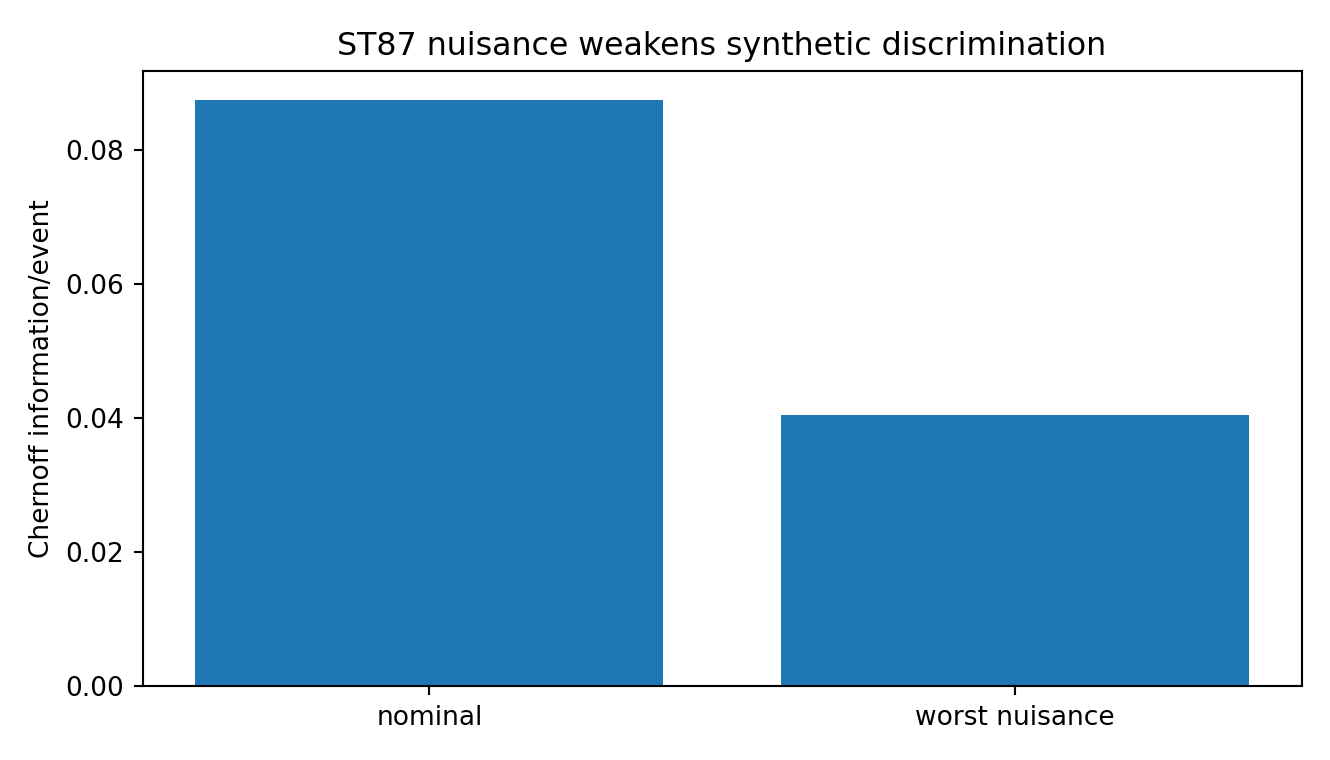
\includegraphics[width=0.70\textwidth]{FIN_ST82_ST93_Figures/st87_robust_likelihood.png}
\caption{Declared contamination substantially reduces synthetic discrimination. This is an optimized model rate, not a laboratory count guarantee.}
\end{figure}

The physical boundary is unchanged: both carriers, their mismatch, the nuisance law, preparations and readout are local synthetic objects. ST87 improves statistical methodology but creates no experimental evidence.

\section{ST88--ST89: irreversible observation and thermodynamic caution}

\subsection{Full-space irreversibility and quotient reversibility}

The strict spectrum has multiplicities $(1,2,2,2,2,2,1)$. Its equal-energy algebra is
\[
\mathcal B=\mathbb C\oplus M_2^5\oplus\mathbb C,
\qquad \dim_{\mathbb C}\mathcal B=22.
\]
Spectral pinching $\Pi:M_{12}\to\mathcal B$ therefore has kernel dimension
\[
12^2-22=122.
\]
Every ST75 unitary-to-dephasing intertwiner factors through $\Pi$. It cannot possess a CPTP inverse on all of $M_{12}$. On $\mathcal B$, however, reversible channels are the $*$-automorphisms
\[
\operatorname{Aut}(\mathcal B)\cong S_2\times\bigl(PU(2)^5\rtimes S_5\bigr).
\]

\begin{figure}[H]\centering
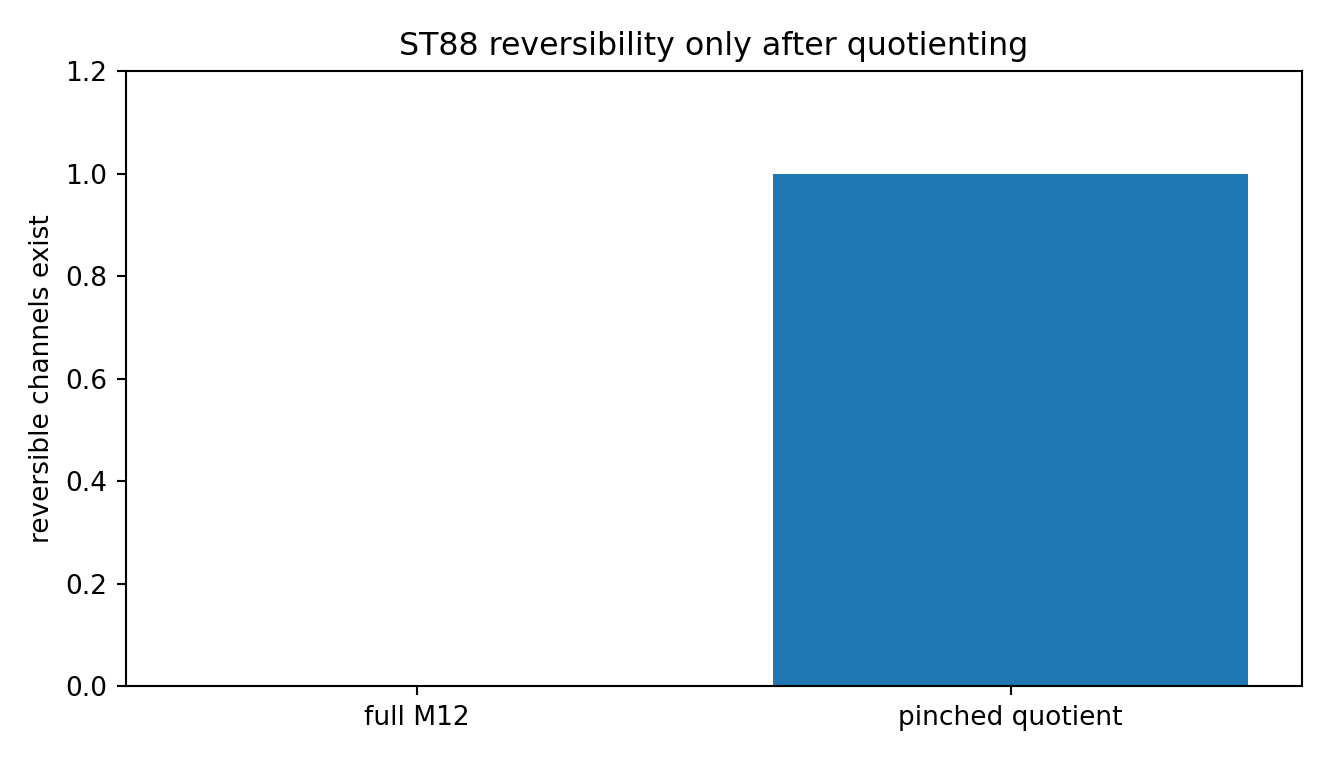
\includegraphics[width=0.66\textwidth]{FIN_ST82_ST93_Figures/st88_reversible_faces.png}
\caption{Reversibility is impossible on the full matrix algebra but exists after restricting to the pinched quotient.}
\end{figure}

This gives a precise mathematical version of ``observation discards information.'' It does not prove that physical observation is spectral pinching. It also shows that an operational quotient can have its own internal symmetries after information has been lost.

\subsection{Gibbs preservation is not thermal physics}

Take a two-level Gibbs state $\gamma=\operatorname{diag}(g_0,g_1)$. Choose positive density matrices $\sigma_0,\sigma_1$ with opposite coherences so that
\[
g_0\sigma_0+g_1\sigma_1=\gamma.
\]
The measure-and-prepare channel
\[
\Phi(\rho)=\rho_{00}\sigma_0+\rho_{11}\sigma_1
\]
is CPTP and Gibbs preserving. But $\Phi(|0\rangle\langle0|)=\sigma_0$ has nonzero energy coherence. It is not time-translation covariant, while energy-conserving thermal operations are covariant. Therefore
\[
\boxed{\text{thermal operations}\subsetneq\text{Gibbs-preserving channels}.}
\]
The numerical positivity and fixed-point residuals are independently checked. This counterexample prevents the report from interpreting an arbitrary Gibbs-preserving FIN channel as thermodynamic dynamics.

\section{ST90--ST91: nonlinear multiplicity and conditional stability}

ST90 runs 80 reflection-reduced multistarts at each of five couplings. It finds 34, 31, 23, 5 and 3 distinct sorted-amplitude signatures at $\kappa=0.02,0.05,0.1,0.5,1.0$, respectively. These counts are lower bounds on solutions reached by the solver, not exact branch counts.

\begin{figure}[H]\centering
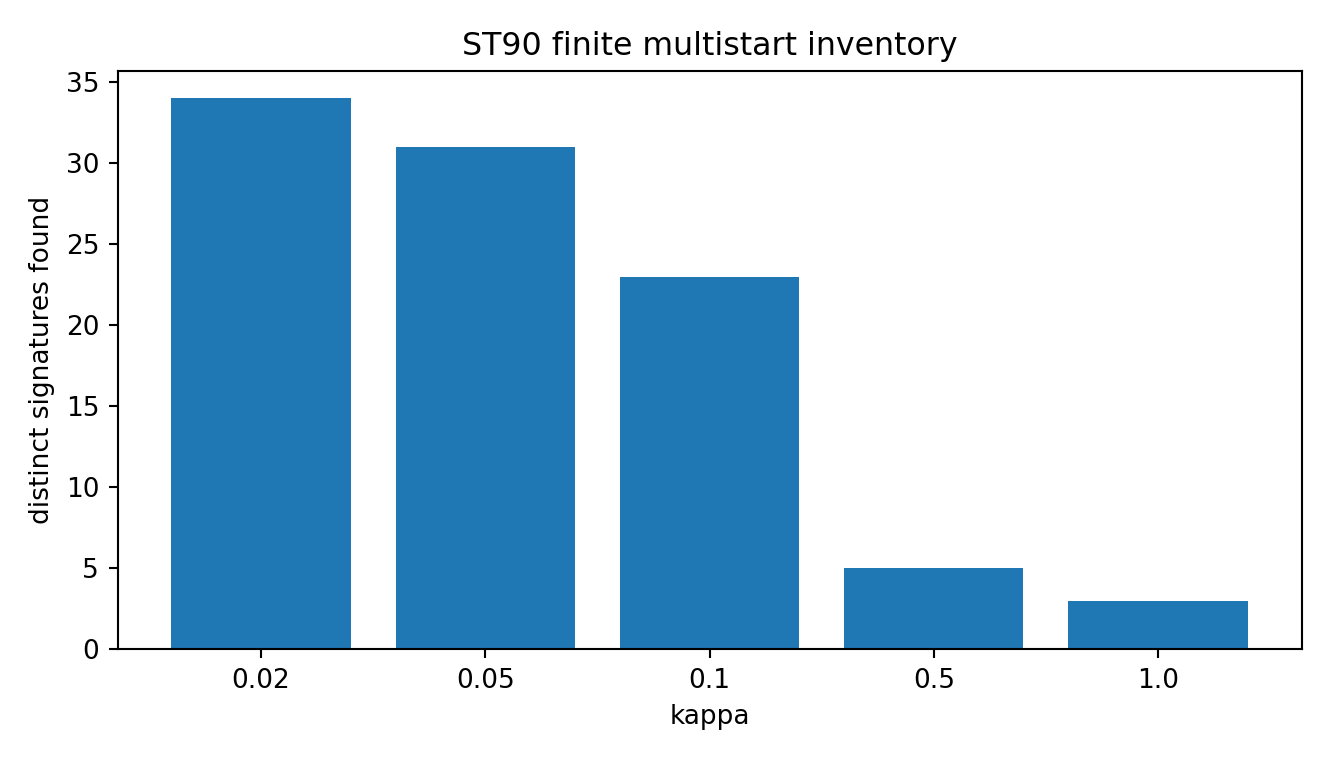
\includegraphics[width=0.70\textwidth]{FIN_ST82_ST93_Figures/st90_branch_inventory.png}
\caption{Finite numerical inventory of reflection-reduced stationary signatures. The decrease with coupling is suggestive but not a theorem.}
\end{figure}

ST91 studies the constructed ST66/ST78 order parameter under an added gradient-flow dynamics. Its linear radial rate at the origin is
\[
\mu-g\lambda_1.
\]
Consequently the origin is unstable for $g<g_c=\mu/\lambda_1$ and stable for $g>g_c$, while the twelve nonzero branches exist on the lower-coupling side.

\begin{figure}[H]\centering
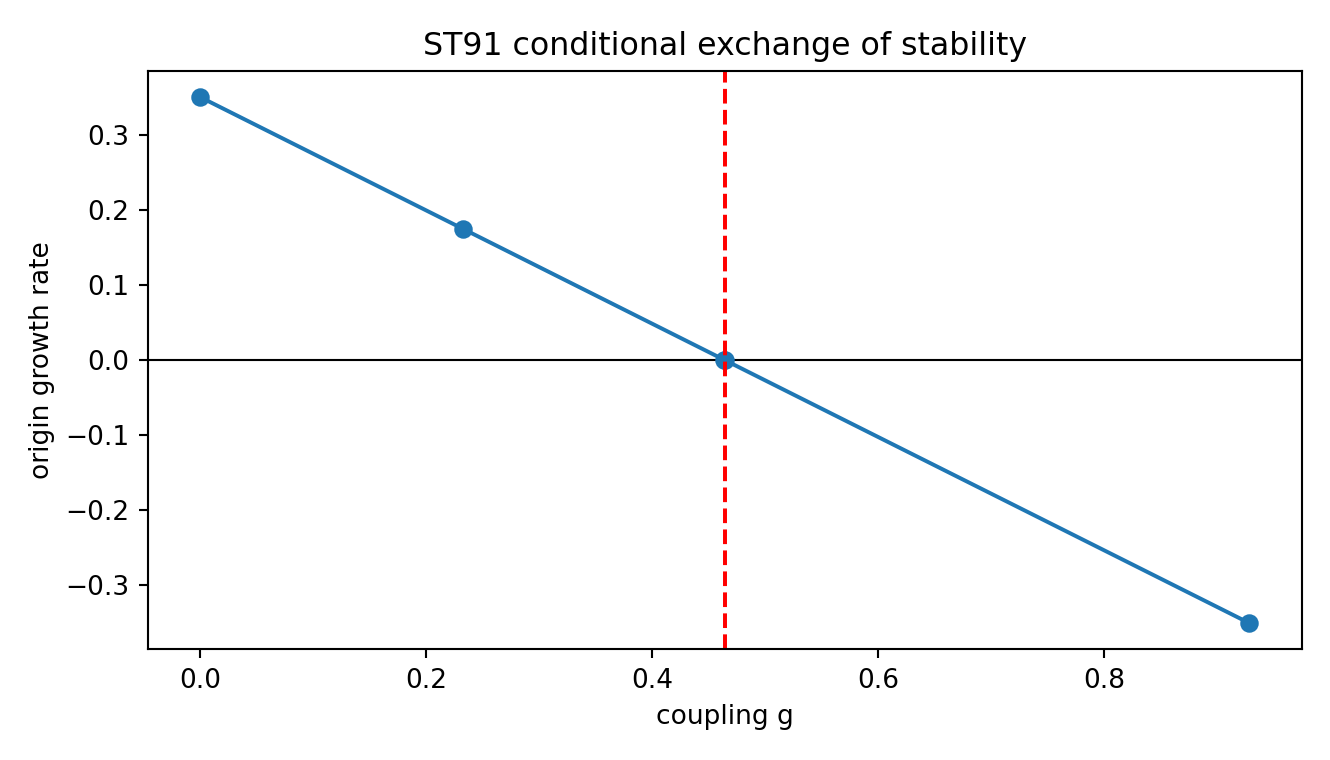
\includegraphics[width=0.70\textwidth]{FIN_ST82_ST93_Figures/st91_dynamic_threshold.png}
\caption{Conditional exchange of local stability in the constructed order-parameter model.}
\end{figure}

This is a valid mechanism of symmetric possibilities, instability, selection, and new stable phases. It makes the user's ``symmetry as a reservoir of possibilities'' intuition mathematically concrete. It does not establish that symmetry itself is positive feedback. The feedback law, potential, gradient metric and clock are added; the strict operator supplies only the stiffness $\lambda_1$.

\section{ST92: strict scalar algebra cannot create an orientation}

Let $R$ be reflection on $C_{12}$. Since $RAR=A$, every polynomial obeys
\[
Rf(A)R=f(A).
\]
Because $A$ is circulant, every diagonal contraction $\operatorname{diag}(A^k)$ is a scalar multiple of the identity. Polynomial commutators vanish. ST92 exhausts the finite class
\[
\{A^0,\ldots,A^{12}\}\cup\{\operatorname{diag}(A^k)\}\cup\{[A^j,A^k]\}.
\]
Its exact span has dimension seven, the number of distinct strict eigenvalues, and its reflection-odd component is exactly zero. Floating relative residuals are below $3.1\times10^{-16}$.

\begin{theorem}[Declared-class selector no-go]
No nonzero reflection-odd object, directed unit, chirality, or strict selector can be generated by the declared scalar polynomial/diagonal/commutator class.
\end{theorem}

This result preserves QW-2191. A state-dependent nonlinear tensor, boundary, record or new typed object may escape the class, but must be explicitly sourced. The conclusion is not that symmetry is undesirable. It is that a deterministic construction preserving the entire stabilizer cannot choose one member of a symmetry orbit.

\section{ST93: dependency graph for the projection interpretation}

The machine-readable file \texttt{FIN\_ST93\_Projection\_Dependency\_Schema.json} records the following architecture:
\[
\begin{array}{c}
W_0\longrightarrow\{\text{projection fiber},\text{irreversible quotient}\},\\[2mm]
(W_0+\text{boundary class})\longrightarrow\text{projective/spin lift},\\[2mm]
\text{selector source}\longrightarrow\text{chosen branch},\\
(W_0+\text{clock})\longrightarrow\text{dimensionful time},\\
(W_0+\text{unit})\longrightarrow\text{dimensionful scale},\\
(\text{preparation,instrument,record})\longrightarrow\text{operational observation}.
\end{array}
\]
The DAG is acyclic and has six explicitly missing source nodes: selector source, clock calibration, physical unit, preparation, calibrated instrument/apparatus, and independent record. A seventh independent resource---the boundary/state class---exists mathematically but is not selected by strict $W_0$.

\begin{figure}[H]\centering
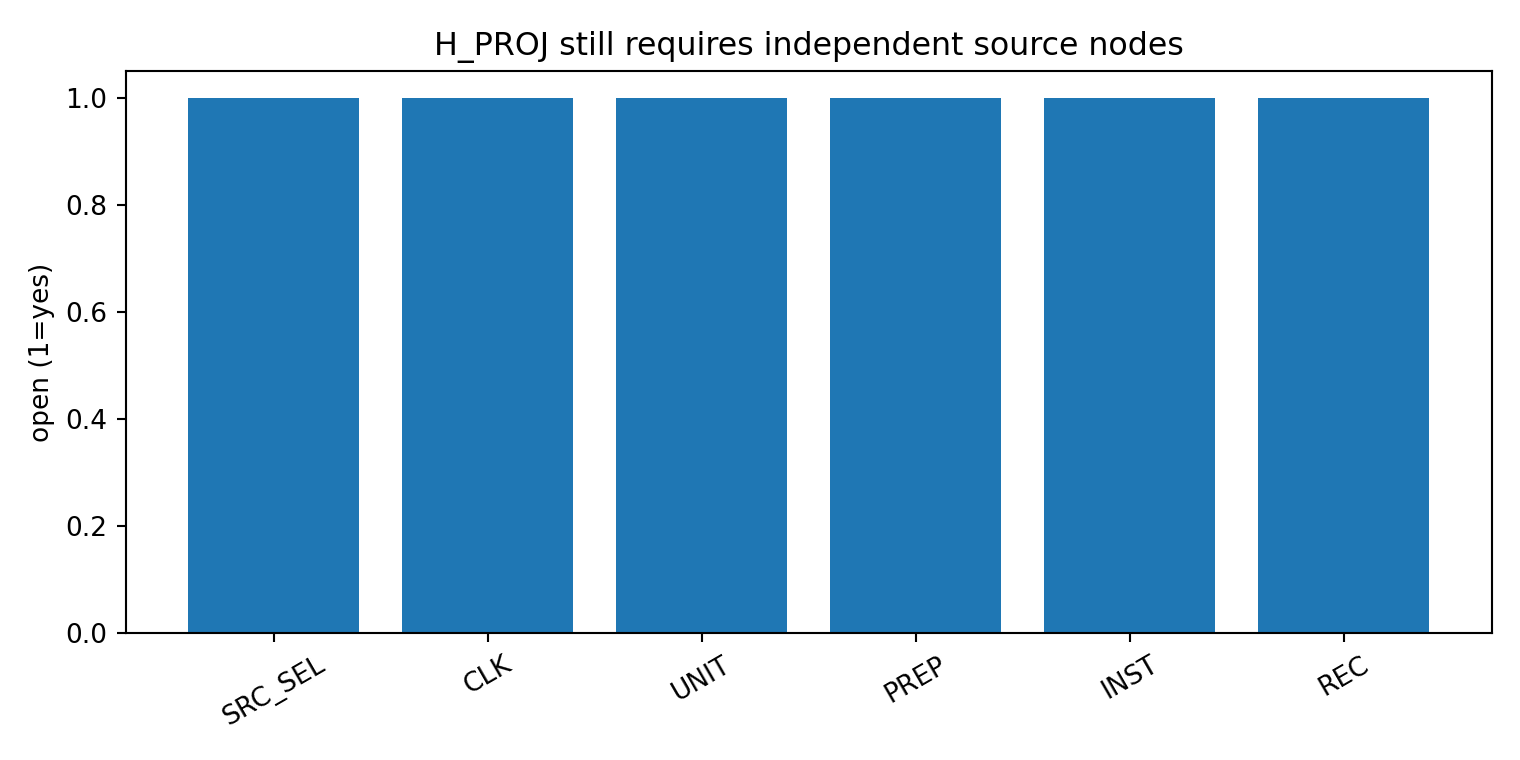
\includegraphics[width=0.86\textwidth]{FIN_ST82_ST93_Figures/st93_missing_sources.png}
\caption{Open source nodes required before the counterfactual projection architecture becomes an operational physical theory.}
\end{figure}

\section{Falsification ledger for the projected-universe reading}

\begin{longtable}{@{}p{0.28\textwidth}p{0.18\textwidth}p{0.46\textwidth}@{}}
\toprule Claim & Verdict & Reason\\\midrule\endfirsthead
\toprule Claim & Verdict & Reason\\\midrule\endhead
A finite deeper object can project to strict dynamics & \proven{} & ST86 constructs an exact reducing coarse sector\\
The projection preserves all channel shadows of $A$ & \proven{} & Functional calculus gives $P^*f(A_{24})P=f(A_{12})$\\
Coarse dynamics determine the deeper object & Refuted & A continuous $q$-fiber is exactly invisible\\
Information loss can be mathematically irreversible & \proven{} & ST88 pinching has kernel dimension 122\\
Irreversibility alone proves an observer & Refuted & No apparatus, record or observer state is generated\\
Passive FIN memory generates active temporal gain & Refuted in class & ST84 complete monotonicity/passivity theorem\\
Scalar strict symmetry selects a spin lift & Refuted in class & ST85 and ST92 retain the boundary/selector source\\
Gibbs preservation is sufficient for thermal physics & Refuted & ST89 GP channel violates time covariance\\
Constructed symmetry breaking proves FIN selects reality & Refuted & ST91 mechanism uses an added potential, metric and clock\\
Present results establish a projected physical universe & Not established & Selection, scale and operational bridge remain absent\\
\bottomrule
\end{longtable}

The strongest surviving interpretation is therefore narrower than the original suggestion:
\begin{quote}
FIN's finite spectral core admits exact coarse-graining maps under which multiple inequivalent finer realizations have identical observable spectral dynamics. This makes projection a natural mathematical language for the model, but not a uniquely selected ontology or a tested physical fact.
\end{quote}

\section{Recommended programs ST94--ST105}

\begin{enumerate}
\item[\textbf{ST94}] \textbf{Projection uniqueness from operational sufficiency.} Add one sharply stated sufficiency/minimality axiom and prove whether it selects a unique conditional expectation. Highest conceptual priority.
\item[\textbf{ST95}] \textbf{Complete lift fiber.} Classify all positive $24\times24$ graph generators satisfying $A_{24}P=PA_{12}$, not only the one-parameter dyadic family.
\item[\textbf{ST96}] \textbf{Petz recovery frontier.} Determine exactly which projected states/coherences are recoverable and characterize equality in data processing.
\item[\textbf{ST97}] \textbf{State-dependent selector.} Construct one equivariant nonlinear state law and test whether bifurcation can choose an orbit member without silently assuming orientation; audit against QW-2191.
\item[\textbf{ST98}] \textbf{Active-memory source.} Seek a strictly derived nonequilibrium signed-residue component, or strengthen ST84 to a larger passive realization class.
\item[\textbf{ST99}] \textbf{Interval fold certificate.} Build outward enclosures of the complete ST83 Jacobian and a verified inverse/preconditioner.
\item[\textbf{ST100}] \textbf{Spin-refinement tower.} Classify periodic/projective compatibility under $12\to24\to48$ and identify every extra boundary choice.
\item[\textbf{ST101}] \textbf{Fine-observable identifiability.} Derive the minimum deliberately non-coarse measurement needed to identify $q$ and prove information bounds.
\item[\textbf{ST102}] \textbf{$C^*$-algebra tower.} Express repeated projections as conditional expectations and test Markov commuting-square conditions.
\item[\textbf{ST103}] \textbf{Certified nuisance optimization.} Replace ST87 differential evolution by interval global optimization over the entire contamination box.
\item[\textbf{ST104}] \textbf{Thermal hierarchy with degeneracies.} Separate thermal, enhanced thermal, covariant Gibbs-preserving and arbitrary Gibbs-preserving maps for the strict multiplicity pattern.
\item[\textbf{ST105}] \textbf{Projection falsification protocol.} Generate alternatives sharing every coarse channel and identify the smallest record that distinguishes projection mechanisms.
\end{enumerate}

The recommended order is ST94 $\to$ ST95 $\to$ ST96 $\to$ ST97. The first three decide whether ``projection'' has mathematical content beyond arbitrary hidden refinement. ST97 then attacks the separate selector obstruction. Programs requiring heavy exact arithmetic should retain bounded checkpoints and must not be promoted from unfinished computation.

\section{Reproducibility and exact claim boundary}

The machine-readable package contains:
\begin{itemize}
\item \texttt{fin\_st82\_st93\_research.py}: deterministic analysis and figures;
\item \texttt{fin\_st82\_rational\_certificate.py}: unfinished independent rational-regeneration implementation, retained as an auditable failed attempt;
\item \texttt{FIN\_ST82\_ST93\_Results.json} and \texttt{FIN\_ST82\_ST93\_Summary.csv};
\item \texttt{FIN\_ST93\_Projection\_Dependency\_Schema.json};
\item \texttt{test\_fin\_st82\_st93.py}: twenty-three live assertions;
\item eight generated figures and the release manifest with SHA-256 hashes.
\end{itemize}

The exact theorems are analytic finite-dimensional statements: ST84, ST85's classification/nonselection, ST86, ST88, ST89, ST91 conditional on its constructed dynamics, ST92, and ST93's DAG audit. Floating computations illustrate or instantiate those statements but do not carry their proof. ST83, ST87 and ST90 retain numerical status. ST82 remains unfinished and is not counted as a successful independent certificate.

\section{Final conclusion}

The user's projection intuition has produced a genuine mathematical advance: ST86 identifies an exact FIN coarse quotient that preserves the entire functional calculus, while exposing a continuous invisible fine fiber. The result is stronger than a visual analogy and weaker than physical ontology. It says that FIN can encode ``one observable shadow, many deeper realizations.'' It does not say which realization exists, why its coarse sector is observed, or why the quotient should be identified with the universe.

The result also clarifies the role of symmetry. Symmetry supplies an orbit of equivalent possibilities. It is not itself positive feedback. A dynamical instability can amplify a perturbation and stabilize one branch, as ST91 proves for an explicitly constructed model, but the selection law remains additional. Likewise, passive memory supplies retardation but not active gain; a spin cover supplies possible projective phases but not their selection; a pinching supplies irreversible information loss but not an observer; Gibbs preservation supplies a fixed point but not thermodynamics.

\resultbox{\textbf{Deepest surviving interpretation.} FIN is presently a finite spectral-information architecture with exact quotient, channel-duality and hidden-refinement structures. Its mathematics naturally supports a projection language, and ST86 makes that language rigorous. The same mathematics proves that the projection is nonunique and operationally underdetermined. Converting it into a physical claim still requires independently sourced selection, boundary, clock, scale, preparation, apparatus and record.}

No QW-2191 closure, legacy-to-strict completion, legacy role transfer, dimensional source, laboratory evidence, Standard Model, gravity, $L_{\rm total}$, or Theory-of-Everything closure is claimed.

\end{document}
